\chapter{Sistemi di telecomunicazione su canale in fibra ottica}
\section{Introduzione}
I sistemi di telecomunicazione in fibra ottica sono basati sulla trasmissione di radiazione luminosa convogliata in un mezzo trasmissivo con banda passante a frequenze dell'ordine di $\SI{e14}{\hertz}$. La fibra è composta da un \keyword[fibra ottica!nucleo]{nucleo} circondato da un involucro che forma il \keyword[fibra ottica!mantello]{mantello}, realizzati con materiali dielettrici ottenuti con differenti tipi di drogaggio della silice per ottenere diversi indici di rifrazione, e da una \keyword[fibra ottica!guaina]{guaina} protettiva esterna che fornisce robustezza fisica, resistenza meccanica, isolamento termico e protezione dall'umidità.

Un raggio monocromatico di luce che incide con un angolo $\theta_1$ rispetto alla normale alla superficie di separazione di materiali a diverso indice di rifrazione emerge con un angolo $\theta_2$ tale da rispettare la \keyword[fibra ottica!legge di Snell]{legge di Snell}:
\begin{equation}
n_1\Sen{\theta_1}=n_2\Sen{\theta_2}
\end{equation}

\begin{figure}[!ht]
\centering
\subfloat{
\begin{tikzpicture}[>=latex',scale=.8]
\fill[pattern=north west lines](-6,-1)rectangle(6,-1.5);
\fill[pattern=north west lines](-6,1)rectangle(6,1.5);
\draw(-6,-1)--(6,-1)(-6,-1.5)--(6,-1.5)(-6,1)--(6,1)(-6,1.5)--(6,1.5);
\draw[dashed](-6,0)--(6,0);
\draw[->](-6,0)--(-3,1);
\draw[->](-3,1)--(3,-1);
\draw[->](3,-1)--(6,0);
\node at(0,1.25){$n_2$};
\node at(0,-1.25){$n_2$};
\node at(0,0.5){$n_1$};
\end{tikzpicture}}\quad\subfloat{
\begin{tikzpicture}
\begin{axis}[xscale=.5,scale=.5,xlabel=$n$,ylabel=$r$,xtick=\empty,ytick=\empty,xmin=0,xmax=2.5]
\addplot[black] coordinates {(0,-1.5)(1,-1.5)(1,-1)(2,-1)(2,1)(1,1)(1,1.5)(0,1.5)};
\end{axis}
\end{tikzpicture}
}
\caption{Fibra ottica \keyword[fibra ottica!step index]{step index}}
\end{figure}

Si definisce \keyword[fibra ottica!angolo critico]{angolo critico} $\theta_c$ l'angolo in corrispondenza del quale la radiazione che incide su una superficie con indice di rifrazione $n_2>n_1$ non viene trasmessa nel mantello ma si propaga lungo la superficie di discontinuità dei due materiali (blu in fig.~\ref{fig:legge_Snell}). Se l'angolo di incidenza è maggiore dell'angolo critico (rosso in fig.~\ref{fig:legge_Snell}), per $\theta_1>\theta_c=\f{\arcsen}{n_2/n_1}$, il raggio è deviato al punto da risultare completamente riflesso dalla superficie di separazione rimanendo intrappolato nel nucleo.
\begin{figure}[!ht]
\centering
\begin{tikzpicture}[>=latex',scale=0.8]
\draw(-3,0)--(3,0);
\draw[dashed](0,-2)--(0,2.5);
\draw[<-](0,0)--(120:2.5);
\draw[<-,blue](0,0)--(135:2.5);
\draw[<-,red](0,0)--(150:2.5);
\draw[->](0,0)--(-30:2.5);
\draw[->,blue](0,0)--(0:2.5);
\draw[->,red](0,0)--(30:2.5);
\node at(3,2.5){$n_1$};
\node at(3,-2){$n_2$};
\draw pic{carc=90:120:1:$\theta_1$};
\draw pic{carc=-90:-30:1:$\theta_2$};
\end{tikzpicture}
\caption{Legge di Snell}
\label{fig:legge_Snell}
\end{figure}

La fibra ottica è in grado di comportarsi in modo quasi ideale fino ad alte frequenze in quanto i fenomeni ottici non sono affetti da attenuazioni tipiche dei trasportatori di carica nei materiali conduttori, come le collisioni degli elettroni che causano una resistenza elettrica con dissipazione di energia termica (effetto Joule), e il rallentamento dei portatori per addensamento sulla superficie esterna dei conduttori in presenza di forti campi elettrici (effetto pelle).

La capacità trasmissiva delle fibre ottiche è limitata dall'effetto di \keyword[fibra ottica!dispersione modale]{dispersione modale}. I raggi che si propagano con velocità costante $v$ in un mezzo trasmissivo con indice di rifrazione costante $n=c/v$ percorrono una distanza che cambia in funzione dell'angolo di incidenza: ogni raggio uscirà dal nucleo con un ritardo di propagazione diverso in funzione del numero di riflessioni che ha subito. Per minimizzare la dispersione modale, proporzionale alla lunghezza della fibra, è possibile utilizzare fibre ottiche \keyword[fibra ottica!monomodale]{monomodali} con un nucleo ridotto ad un diametro inferiore ai $\SI{10}{\micro\meter}$ oppure utilizzare fibre \keyword[fibra ottica!graded index]{graded index} con indice di rifrazione che varia con continuità. I raggi vengono curvati nel nucleo piuttosto che essere riflessi da una superficie di separazione netta. Si cerca di compensare il percorso più lungo dei raggi che viaggiano per le regioni esterne della fibra aumentando la velocità di propagazione con un minore drogaggio del materiale. Essendo la velocità di propagazione inversamente proporzionale alla radice quadrata del'indice di rifrazione, è possibile stabilire con precisione la curva di drogaggio.

\begin{figure}[!ht]
	\centering
	\subfloat{
		\begin{tikzpicture}[>=latex',scale=.8,ray/.style={decoration={markings,mark=between positions 0 and 1 step 2cm with {\arrow{stealth}}}}]
		\fill[pattern=north west lines](-6,-1)rectangle(6,-1.5);
		\fill[pattern=north west lines](-6,1)rectangle(6,1.5);
		\draw(-6,-1)--(6,-1)(-6,-1.5)--(6,-1.5)(-6,1)--(6,1)(-6,1.5)--(6,1.5);
		\foreach\i[evaluate=\i as \x using {1/sqrt(1-(\i/10-1)^2)-1.}] in{1,...,9} {
			\draw[dotted](-6,\x)--(6,\x);
			\draw[dotted](-6,-\x)--(6,-\x);
		}
		\draw[ray,postaction={decorate}](-6,0).. controls(-3,1)and(-3,1)..(0,0)
		..controls(3,-1)and(3,-1)..(6,0);
		\draw[ray,postaction={decorate}](-6,0).. controls(-4,1)and(-4,1)..(-2,0)
		..controls(0,-1)and(0,-1)..(2,0) .. controls(4,1)and(4,1)..(6,0);
		\end{tikzpicture}}\quad\subfloat{
		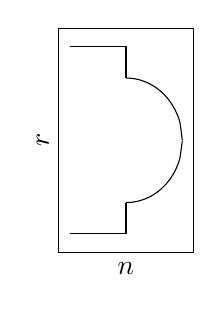
\begin{tikzpicture}[yshift=-4mm]
		\begin{axis}[xscale=0.5,scale=.5,xlabel=$n$,ylabel=$r$,xtick=\empty,ytick=\empty]
		\addplot[black] coordinates {(0,-1.5)(1,-1.5)(1,-1)};
		\addplot[smooth,domain=1:2]{sqrt(1-(x-1)^2)};
		\addplot[smooth,domain=1:2]{-sqrt(1-(x-1)^2)};
		\addplot[black] coordinates {(1,1)(1,1.5)(0,1.5)};
		\end{axis}
		\end{tikzpicture}
	}\caption{Fibra ottica \keyword[fibra ottica!graded index]{graded index}}
\end{figure}

Altri fenomeni ottici comportano problemi come l'efficienza di iniezione, in cui va considerato che solo una quota parte della radiazione emessa dalla sorgente penetra nel nucleo con angolo che porta alla propagazione, che una parte viene persa per assorbimento nel mantello, e viene riflessa o si perde in presenza delle giunzioni. Inoltre si verifica dispersione cromatica per cui diverse componenti spettrali del segnali si propagano a diverse velocità rendendo difficoltosa la ricomposizione del segnale in ricezione.

Bisogna tener conto dei fenomeni di attenuazione in corrispondenza delle lunghezze d'onda alle quali avvengono fenomeni di assorbimento dovuti alle molecole del materiale. In particolare i gruppi ossidrile OH dovuti al residuo di acqua contenuto nella silice causano assorbimento alle lunghezze d'onda di $\SI{1.24}{\micro\meter}$ e $\SI{1.38}{\micro\meter}$.
Tenendo conto dei diversi fenomeni di attenuazione, dispersione, e di ulteriori perdite per diffusione (\emph{scattering di Rayleigh}), restano individuate tre finestre trasmissive adatte all'uso nelle telecomunicazioni, con prestazioni e costi crescenti, senza apparecchiature intermedie per rigenerare il segnale per collegamenti a lunga distanza:
\begin{itemize}
\item la prima finestra a $\SI{850}{\nano\meter}$ nel campo del visibile, utilizzata con fotodiodi e LED al silicio e i primi laser economici a luce multimodale, che consentono collegamenti inferiori al km e una attenuazione $\cong\SI{1}{\decibel\per\kilo\meter}$.
\item la seconda finestra a $\SI{1.33}{\micro\meter}$ utilizzata con laser multimodali e monomodali e collegamenti inferiori ai $\SI{10}{\kilo\meter}$ con attenuazione $\cong\SI{.5}{\decibel\per\kilo\meter}$.
\item la terza finestra a $\SI{1.55}{\micro\meter}$ usata con laser monomodali può raggiungere collegamenti di $\SI{100}{\kilo\meter}$ grazie alla bassissima attenuazione di $\SI{0.2}{\decibel\per\kilo\meter}$.
\end{itemize}

\begin{figure}[!ht]\centering
\begin{tikzpicture}
\begin{axis}[xlabel={$\lambda [\si{\micro\meter}]$},ylabel={$\alpha [\si{\decibel\per\kilo\meter}]$},xtick=\empty,ytick=\empty,extra x ticks={.8,1.33,1.55},extra y ticks={.2,.5,1}]
\addplot[smooth,name path=f1] coordinates {(0.3,2.5) (0.8,1)(1.24,1.25)};
\addplot[smooth,name path=f2] coordinates {(1.24,1.25) (1.33,0.5)(1.38,1.0)};
\addplot[smooth,name path=f3] coordinates {(1.38,1) (1.56,0.22) (2,2.5)};
\draw[help lines,dashed](axis cs:0,1)-|(axis cs:.8,0) (axis cs:0,.5)-|(axis cs:1.33,0) (axis cs:0,.2)-|(axis cs:1.55,0);
\fill[fill=gray!20,fill opacity=.5] (axis cs:.78,0)rectangle(axis cs:1,2.5) node[midway]{$I$};
\fill[fill=gray!20,fill opacity=.5] (axis cs:1.3,0)rectangle(axis cs:1.36,2.5) node[midway]{$II$};
\fill[fill=gray!20,fill opacity=.5] (axis cs:1.49,0)rectangle(axis cs:1.58,2.5) node[midway]{$III$};
\end{axis}
\end{tikzpicture}
\end{figure}

Le sorgenti di radiazione del sistema di trasmissione possono operare a diverse lunghezze d'onda e potenza. Un \ac{LED} ha densità spettrale di potenza del segnale emesso qualitativamente mostrato in figura \ref{fig:densita_potenza_LED} con una larghezza di banda di circa $\SI{100}{\mega\hertz}$.
Una sorgente \ac{LASER} genera la radiazione luminosa in una cavità risonante chiusa tra specchi riflettenti: la radiazione emessa acquista potenza prima di emergere dalla sorgente in modo accentuato alle frequenze di risonanza della cavità (fig.~\ref{fig:densita_potenza_LASER}).Ad un'analisi spettrale risultano ravvicinate tra loro con una larghezza di banda di circa $\SI{10}{\mega\hertz}$ e una banda relativa molto ristretta.

Le velocità di trasmissione su fibre ottiche è limitata dalla capacità delle sorgenti, in particolare i \ac{LED}, di variare il loro stato con transizioni molto rapide.
\begin{figure}[!ht]\centering
	\subfloat[Sorgente LED]{
	\begin{tikzpicture}
	\begin{axis}[hide y axis,axis x line=middle,ymax=1.2,xlabel={$\lambda$},xtick={0},xticklabels={$\lambda_0$},ytick=\empty]
	\addplot[domain=-3:3,samples=200] {gauss(x,0,1)};
	\end{axis}
	\end{tikzpicture}
	\label{fig:densita_potenza_LED}
	}\quad\subfloat[Sorgente laser]{
	\begin{tikzpicture}
	\begin{axis}[hide y axis,axis x line=middle,xlabel={$\lambda$},xtick={0},xticklabels={$\lambda_0$},ytick=\empty]
	\addplot[samples=400] {gauss(x,0,1)/(.2+(sin(5*x))^2)};
	\end{axis}
	\end{tikzpicture}
	\label{fig:densita_potenza_LASER}
	}
	\caption{Densità spettrale di potenza del segnale emesso da sorgenti di radiazione \ac{LED} e \ac{LASER}}
\end{figure}

\section{Dimensionamento}
Un sistema di trasmissione su fibra ottica è costituito da un trasmettitore con una sorgente di radiazione luminosa con modulazione \ac{OOK} e un ricevitore dotato di un fotorivelatore che trasforma la potenza ottica 
\begin{figure}[!ht]
	\centering
	\resizebox{\textwidth}{!}{
		\begin{tikzpicture}[>=latex',fitted/.style={draw,thick,dotted,inner sep=4mm,rounded corners}]
		\coordinate(c0);
		\node[block,right=1.5cm of c0](b0){OOK};
		\node[block,right=1.5cm of b0,minimum height=1em](f0){fibra}edge[<-](b0);
		\node[block,right=1cm of f0](b1){PIN}edge[<-](f0);
		\node[draw,right=1cm of b1,thick,isosceles triangle,minimum height=1cm](b2){}edge[<-](b1);
		\node[block,right=1cm of b2](b3){DEM}edge[<-](b2);
		\node[block,right=1cm of b3](b4){$H_R$}edge[<-](b3);
		\node[campionatore,right=1cm of b4](q0){}edge[<-](b4);
		\node[block,right=1cm of q0](b5){DEC}edge[<-](q0);
		\coordinate[right=1.5cm of b5](c1);
		\draw[->](c0)--node[above,near start]{bit}(b0);
		\draw[->](b5)--node[above,near end]{bit}(c1);
		\node[fitted, fit=(b0),label=above:Trasmettitore]{};
		\node[fitted, fit=(b1)(b2)(b3)(b4)(b5),label=above:Ricevitore]{};
		\node[fitted, fit=(f0),label=above:Canale]{};
		\draw [section={$P_T$}] (b0)--(f0);
		\end{tikzpicture}
	}
	\caption{Schema di trasmissione in fibra ottica}
\end{figure}